\documentclass[11pt]{article}

\usepackage[a4paper,margin=23mm]{geometry}
\usepackage[T1]{fontenc}
\usepackage{amsmath,amssymb,bm}
\usepackage{booktabs,longtable,tabularx,array}
\usepackage{graphicx}
\usepackage{xcolor}
\usepackage{enumitem}
\usepackage{hyperref}
\usepackage{url}

\hypersetup{
  colorlinks=true,
  linkcolor=blue!55!black,
  urlcolor=blue!55!black,
  citecolor=blue!55!black,
  pdftitle={Chapter 13 Wilson Adiabatic Qualification Synthesis},
  pdfauthor={Aion development record}
}
\setlist{nosep,leftmargin=*}
\setcounter{tocdepth}{2}
\renewcommand{\arraystretch}{1.14}
\setlength{\tabcolsep}{3pt}
\emergencystretch=2em
\newcolumntype{Y}{>{\raggedright\arraybackslash}X}
\newcommand{\iu}{\mathrm{i}}
\newcommand{\dd}{\mathrm{d}}
\newcommand{\Tr}{\operatorname{Tr}}
\newcommand{\ReTr}{\operatorname{Re}\operatorname{Tr}}
\newcommand{\A}{\mathbf A}
\newcommand{\B}{\mathbf B}
\newcommand{\E}{\mathbf E}
\newcommand{\rvec}{\mathbf r}
\newcommand{\Smat}{\mathbf S}
\newcommand{\Kmat}{\mathbf K}
\newcommand{\Pmat}{\mathbf P}
\newcommand{\Dmat}{\mathbf D}
\newcommand{\omegamat}{\boldsymbol\omega}
\newcommand{\status}[1]{\textsf{#1}}

\title{\textbf{Chapter 13 Wilson Adiabatic Qualification in Aion}\\
\large Final NQ9 synthesis, numerical evidence, and Chapter 14 handoff}
\author{Aion development record}
\date{24 September 2026}

\begin{document}
\maketitle

\begin{center}
\fbox{\begin{minipage}{0.92\textwidth}
\textbf{Status.} NQ0--NQ8 have separate user-accepted review records.  The
NQ9 synthesis reported here was executed and authenticated, but NQ9 itself is
\status{unreviewed}.  No statement in this document changes a mathematical
source or extends the accepted physical domain.  Raw executions remain
immutable; scientific acceptance is carried only by review records.
\end{minipage}}
\end{center}

\vspace{0.5em}
\noindent\textbf{Repository branch:}
\path{feature/ch13-wilson-adiabatic-qualification}.\\
\textbf{NQ9 synthesis commit:} \texttt{74a493241667}.\\
\textbf{Synthesis result SHA-256:}\\
\path{4eca05f7fbf774a0a47a6d44146929d35941f7fb013acfa6ace973c5080c6671}.

\tableofcontents
\listoffigures
\listoftables
\clearpage

\section{Purpose and evidentiary rules}

This report is the principal human-readable entry point to the fixed-centre
Wilson Hartree and adiabatic Kohn--Sham qualification campaign.  It answers
the seven questions required by NQ9: which claims have direct numerical
support; the systems, bases, fields, functionals, and times over which they
were tested; the numerical floor on each claim; the supported reduced
electromagnetic action; the observed metric, density-domain, auxiliary,
grid, nonlinear, and propagation failures; their basis dependence; and the
questions deferred to broader physics.

Four kinds of statement remain distinct throughout:

\begin{description}[style=nextline]
  \item[Mathematical identity]
  A statement following from the declared continuum action, Wilson frame,
  and index conventions.  It does not assert that code exists.
  \item[Reusable implementation]
  A versioned Aion API.  Its presence does not imply that the accepted
  calculation exercised it.
  \item[Executed evidence]
  A calculation tied to code, environment, fixture, precision, and immutable
  hashes.  Execution alone does not accept the scientific interpretation.
  \item[Reviewed evidence]
  An explicit user decision in \path{docs/reviews}.  Only this state accepts
  a gate and authorizes the next one.
\end{description}

The independent NQ9 synthesis read the nine NQ0--NQ8 review records,
authenticated 41 primary artifacts, flattened 131 accepted measurements and
49 declared limitations, materialized 13 equation-to-code-to-evidence rows,
and retained eight explicit negative results.  It did not rerun or rewrite
any scientific campaign.

\section{Physical and mathematical model}

\subsection{Fixed Wilson frame and density variables}

The accepted problem uses fixed nuclei and fixed Gaussian AO anchors
$\{\mathbf R_i\}$.  A straight Wilson path dresses each AO,
\begin{equation}
  \chi_i^W(\rvec,t)
  =\exp\!\left[\frac{\iu q}{\hbar}
    \int_{\mathbf R_i}^{\rvec}\A(\boldsymbol\ell,t)\cdot\dd\boldsymbol\ell
  \right]\phi_i(\rvec).
\end{equation}
The finite-frame overlap and exact Wilson density are
\begin{align}
 S_{ij}(t)&=\langle\chi_i^W(t)|\chi_j^W(t)\rangle,\\
 n_W(\rvec,t)&=P^{ij}(t)\chi_i^W(\rvec,t)\chi_j^W(\rvec,t)^*.
\end{align}
Here $\Pmat=C f C^\dagger$ is the contravariant coefficient density.  The
mixed tensor $\Dmat=\Pmat\Smat$ exposes trace, occupation spectrum, and
metric geometry.  $P$ and $D$ are not interchangeable in AO contractions.

NQ1 establishes direct versus endpoint/triangle-factorized density
agreement, unrestricted real and imaginary coefficient derivatives,
fixed-history vector-potential derivatives, magnetic-gauge representative
invariance, general complex nonunitary coefficient-frame covariance, and
CPU/GPU parity.  The largest direct/factorized relative difference is
$2.54\times10^{-16}$; the finest accepted real-space normalization floor is
$2.32\times10^{-11}$.

\subsection{One common nonlinear action}

The exact finite-subspace Hartree and adiabatic Kohn--Sham branches use
\begin{align}
 U_H[P,A] &= \Tr(PK_{1e})+E_H[n_W]+E_{NN},\\
 U_{KS}[P,A] &= \Tr(PK_{1e})+E_H[n_W]+E_{xc}[n_W]+E_{NN}.
\end{align}
The scalar-potential coupling belongs to the temporal connection and is not
added a second time to these mechanical energies.

The Coulomb-metric RI realization is a single discrete action,
\begin{equation}
 E_H=\frac12\rho_A(J^{-1})^{AB}\rho_B,
\end{equation}
whose lower matrix and fixed-history source derivative are analytic
derivatives of the same fitted energy.  The selected auxiliary basis is an
explicit approximation: its largest accepted deviation from an independent
four-centre reference is $6.90\times10^{-5}$ relative.  It must therefore be
called ``RI--Wilson Hartree'', not exact Coulomb.

For LDA, the quadrature action is
\begin{equation}
 E_{xc,Q}=\sum_g w_g f(n_W(\rvec_g)).
\end{equation}
For GGA it is separately labelled and extended to
\begin{equation}
 E_{xc,Q}=\sum_g w_g f(n_W(\rvec_g),\nabla n_W(\rvec_g)).
\end{equation}
Energy, weak lower matrix, and source derivative reuse the same nodes,
weights, dressed AO values, dressed gradients, screening rules, and
pointwise libxc data.  The GGA source derivative includes both
$\delta_A n_W$ and $\delta_A\nabla n_W$.  LDA evidence is never relabelled as
GGA evidence.

\subsection{Stationary equation and source observables}

At fixed prescribed source, the occupied orbitals obey the nonlinear
generalized Hermitian equation
\begin{equation}
 K[P]C=SC\varepsilon,
\end{equation}
with fixed closed-shell occupations.  The implementation monitors orbital,
density fixed-point, mixed-commutator, metric-orthonormality, particle-number,
occupation-spectrum, energy-stationarity, and double-counting residuals.

A vector-source test $\alpha$ differentiates the complete action at fixed
coefficient history.  The off-shell response separates into minimal,
tangential, embedding, and normal-subspace terms.  On the coefficient shell,
the tangential virtual work vanishes, leaving the action-derived physical
weak pairing.  No ambient momentum current, graph current, P0 current, or
observable from a different approximation is substituted.

The same source construction yields the off-shell Ward identity and the
on-shell weak continuity relation
\begin{equation}
 \frac{\dd}{\dd t}\int f(\rvec)q n_W(\rvec,t)\,\dd\rvec
 =\langle j_{\rm action}(t),\nabla f\rangle.
\end{equation}
The constant-weight limit tests global signed-charge conservation.  For a
Kohn--Sham branch, this is the source current of the declared auxiliary
adiabatic action; no exact interacting transverse current is claimed.

\subsection{Connection-aware nonlinear propagation}

The moving finite Wilson frame supplies the exact overlap, temporal
connection, and complete lower mechanical matrix:
\begin{align}
 S\dot C&=-\left(\omega+\frac{\iu}{\hbar}K[P,t]\right)C,\\
 G[P,t]&=S^{-1}\left(-\omega-\frac{\iu}{\hbar}K[P,t]\right),\\
 \dot S&=\omega+\omega^\dagger.
\end{align}
The connection is evaluated from the prescribed electromagnetic source; it
is not reconstructed from $\dot S$.  Metric compatibility is checked
independently.

For each step, the accepted integrator evaluates the nonlinear generator at
the two fourth-order Gauss nodes
$c_\pm=1/2\pm\sqrt{3}/6$.  Self-consistent node densities define
\begin{equation}
 \Omega=\frac h2(G_-+G_+)-\frac{\sqrt3h^2}{12}[G_-,G_+],
\end{equation}
whose exponential is approximated by the diagonal $[2/2]$ Pad\'e map $U$.
The endpoint update is the congruence
\begin{equation}
 P_{n+1}=U P_n U^\dagger,
\end{equation}
followed by $D_{n+1}=P_{n+1}S_{n+1}$.  There is no L\"owdin coordinate
transformation, Cholesky endpoint correction, metric projection, clipping,
or density repair.  Cross-metric, trace, and occupation defects remain
visible and converge with timestep.

The matrix-rate and action-source power routes independently test
\begin{equation}
 U(T)-U(0)=\int_0^T\langle j_{\rm action}(t),E(t)\rangle\,\dd t.
\end{equation}
A time-dependent uniform magnetic field is always accompanied by its affine
induction electric field.

\section{Reusable implementation and PySCF boundary}

PySCF supplies molecular geometry, all-electron Gaussian bases, bare AO and
auxiliary integrals, molecular quadrature grids, AO values and derivatives,
field-free RHF/RKS references, and pointwise libxc values.  Aion owns the
anchors, Wilson phases and gradients, complex pair contractions, exact
finite-frame matrices and connection, RI--Wilson action, LDA/GGA action
derivatives, nonlinear composition, action-source observables, and time
propagation.

\begin{longtable}{p{0.25\textwidth}p{0.67\textwidth}}
\caption{Principal reusable Aion implementation.}\label{tab:implementation}\\
\toprule
Object & Module and responsibility\\
\midrule
\endfirsthead
\toprule
Object & Module and responsibility\\
\midrule
\endhead
Wilson density & \path{electronic_structure/wilson_density.py}: blocked exact density and matter/source directions\\
RI Hartree & \path{electronic_structure/ri_wilson_hartree.py}: fitted action, lower matrix, and source derivative\\
LDA action & \path{electronic_structure/wilson_lda.py}: common quadrature energy and derivatives\\
GGA action & \path{electronic_structure/wilson_gga.py}: dressed gradients and common PBE action derivatives\\
Stationary model & \path{electronic_structure/wilson_stationary.py}: Hartree/LDA/GGA action composition and generalized SCF\\
Weak sources & \path{electronic_structure/wilson_sources.py}: charge, current decomposition, Ward identity, and continuity\\
Dynamic model & \path{electronic_structure/wilson_dynamics.py}: source samples, nonlinear EOM triple, and power\\
Reduced actions & \path{electronic_structure/reduced_wilson.py}: P0, E1, strict C1, and resummed C1\\
Time connection & \path{electronic_structure/time_connection.py}: exact connection, metric rate, and source directions\\
Propagator & \path{propagation/tensorial.py}: self-consistent contravariant-density Gauss--Magnus evolution\\
\bottomrule
\end{longtable}

GPU execution keeps Wilson frames and matrix contractions device-resident.
Only real pointwise libxc inputs and outputs cross the host boundary.  The
physical-GPU launcher rejects a missing device or silent CPU fallback.  NQ8's
complete final GPU regression contained 31 passing tests and one expected
CuPy contraction-engine warning.

\section{Gate-by-gate evidence}

\begin{longtable}{p{0.07\textwidth}p{0.26\textwidth}p{0.43\textwidth}p{0.14\textwidth}}
\caption{Accepted NQ0--NQ8 evidence summarized by NQ9.}\label{tab:gates}\\
\toprule
Gate & Qualified object & Central evidence & Main limiting floor\\
\midrule
\endfirsthead
\toprule
Gate & Qualified object & Central evidence & Main limiting floor\\
\midrule
\endhead
NQ0 & Contract and field-free reference & H$_2$/STO-3G LDA realization, density/index ledger, component energy reconstruction & $4.44\times10^{-16}$ Ha energy closure\\
NQ1 & Exact Wilson density & H$_2$ and LiH density, matter/source directions, gauge and frame covariance & $2.32\times10^{-11}$ grid normalization\\
NQ2 & RI--Wilson Hartree & Independent four-centre reference; grid, auxiliary, rank, solve, matter, and source scans & $6.90\times10^{-5}$ selected auxiliary relative error\\
NQ3 & Wilson LDA & Same-grid PySCF/libxc reference, unrestricted derivatives, gauge/frame covariance & $3.27\times10^{-9}$ Ha level-4 to level-5 grid energy\\
NQ4 & Stationary states & H$_2$ recovery and H$_3^+$ field scan through $B_z=0.06$ & $6.53\times10^{-9}$ Ha grid and stationarity floor\\
NQ5 & Sources and continuity & Complete action derivative, Gauss decomposition, off-shell Ward and on-shell weak continuity & $1.09\times10^{-9}$ level-5 grid charge\\
NQ6 & Nonlinear dynamics & 56 LDA/Hartree trajectories, timestep and nonlinear refinement, power/work identities & $6.97\times10^{-8}$ finest density step difference\\
NQ7 & Reduced actions & P0/E1/C1 exact comparisons and three-basis domain stress test & basis-conditioned loss of reduced metric positivity\\
NQ8 & PBE and CO transfer & Same-grid PBE, sources, stationary state, continuity, power, and short dynamics & $7.39\times10^{-9}$ CO source derivative\\
\bottomrule
\end{longtable}

The selected systems are H$_2$, LiH, physical two-electron equilateral
H$_3^+$, and closed-shell CO.  Accepted orbital bases are STO-3G and
cc-pVDZ; aug-cc-pVDZ appears only in the reduced-domain stress scan, not as a
general production qualification.  Production fixtures use the weigend
auxiliary basis.  The qualified closures are Hartree only, restricted pure
\texttt{lda,vwn}, and restricted pure PBE.

\section{Numerical results and error separation}

\subsection{Action derivatives and stationary states}

On exactly matched grids, the LDA energy and lower matrix agree with the
independent PySCF/libxc route to $1.33\times10^{-15}$ Ha and
$3.39\times10^{-16}$ relative.  The PBE counterparts agree to
$5.33\times10^{-15}$ Ha and $4.14\times10^{-16}$ relative.  These comparisons
isolate the XC action from the RI and grid choices.

The accepted H$_3^+$ stationary LDA scan has maximum orbital and density
fixed-point residuals $2.49\times10^{-13}$ and $9.04\times10^{-13}$.  Gauge
related energies and real-space densities agree within
$2.90\times10^{-13}$ Ha and $8.61\times10^{-13}$ relative.  For PBE transfer,
the largest field-orbital residual is $3.92\times10^{-12}$ and the minimum
metric eigenvalue is $2.17\times10^{-2}$.

\begin{figure}[htbp]
  \centering
  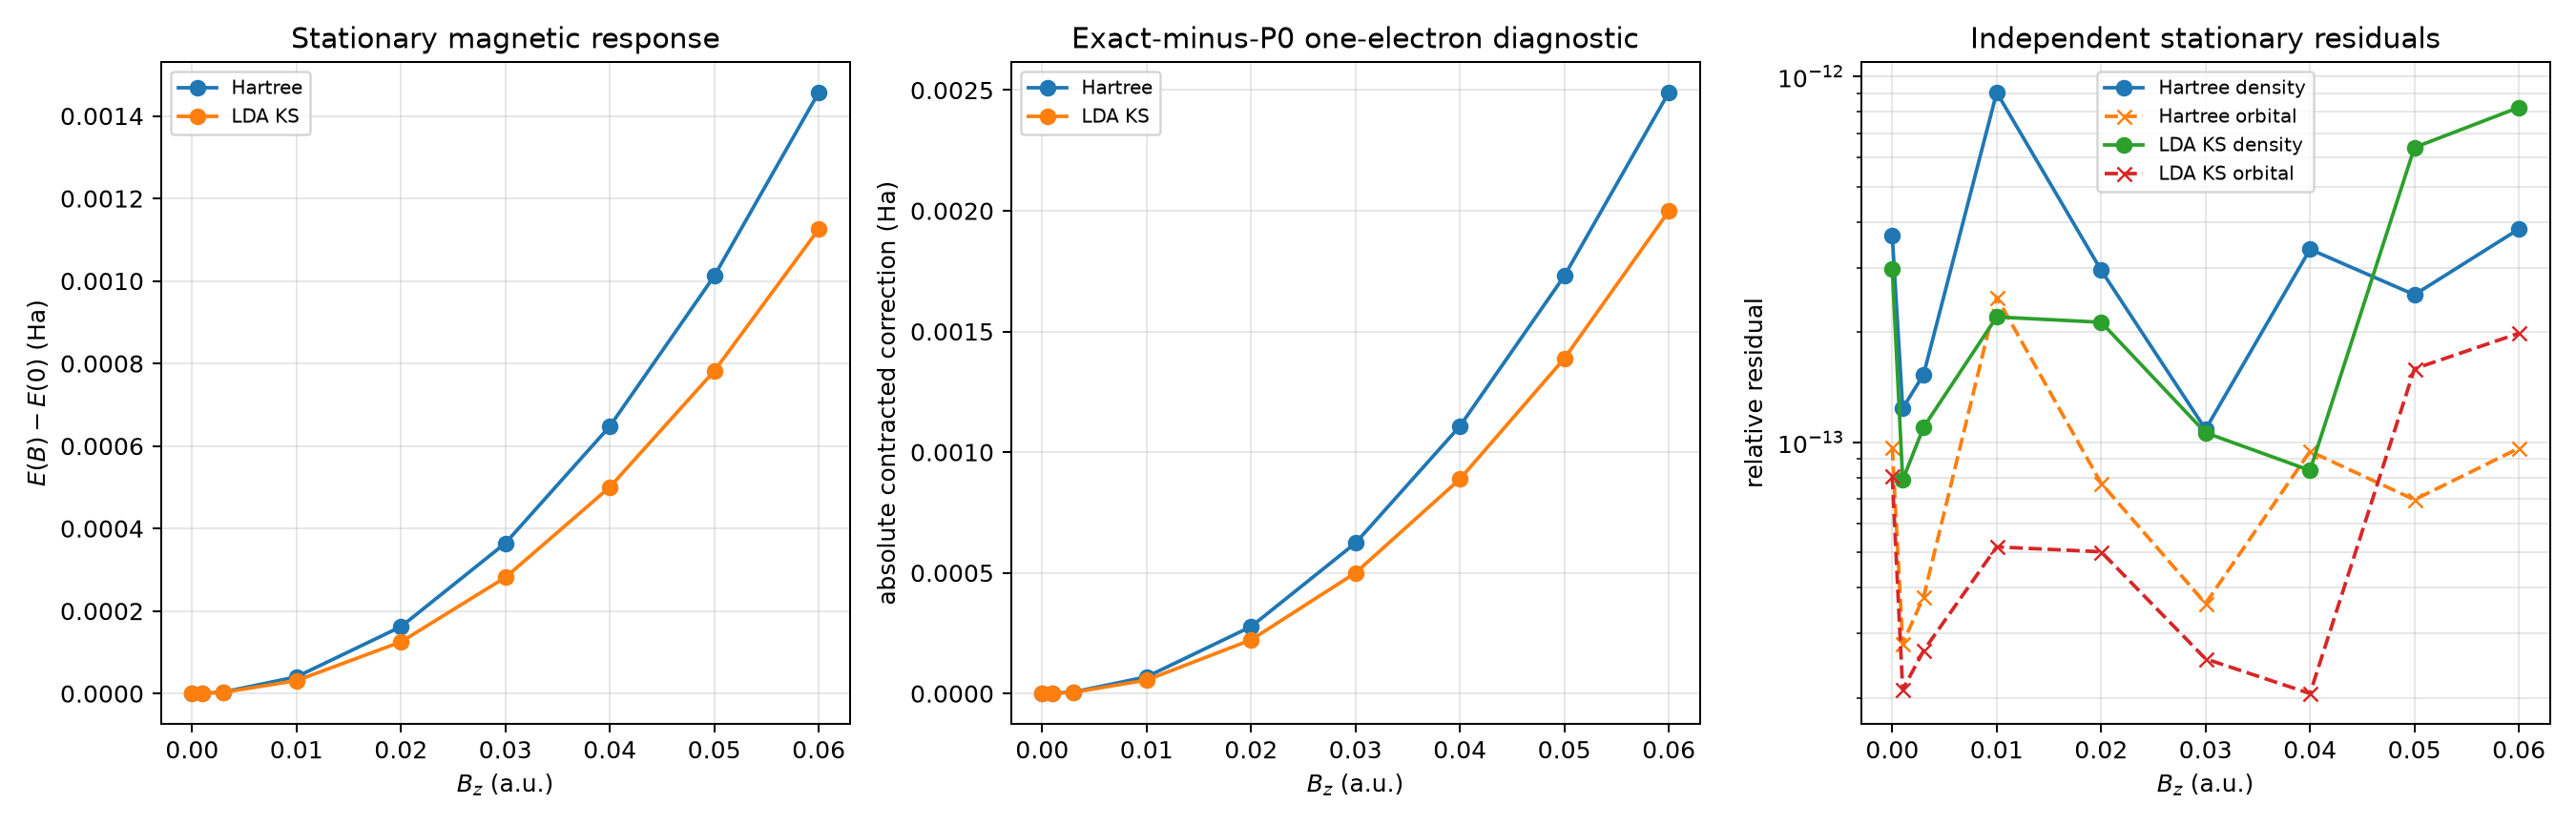
\includegraphics[width=0.88\textwidth]{figures/chapter13_nq9/nq4_h3plus_stationary_field_scan.png}
  \caption{Accepted H$_3^+$ exact-Wilson stationary field scan from NQ4.}
  \label{fig:stationary}
\end{figure}

\subsection{RI, grid, and finite-difference floors}

The Hartree campaign separates real-space quadrature, auxiliary basis,
retained rank, and linear solve.  The finest selected-grid energy and lower
matrix errors are $1.53\times10^{-10}$ and $4.23\times10^{-10}$ relative.
The production solve residual is $5.04\times10^{-13}$, much smaller than the
auxiliary approximation.  This separation prevents a tight solve from being
misreported as exact Coulomb physics.

\begin{figure}[htbp]
  \centering
  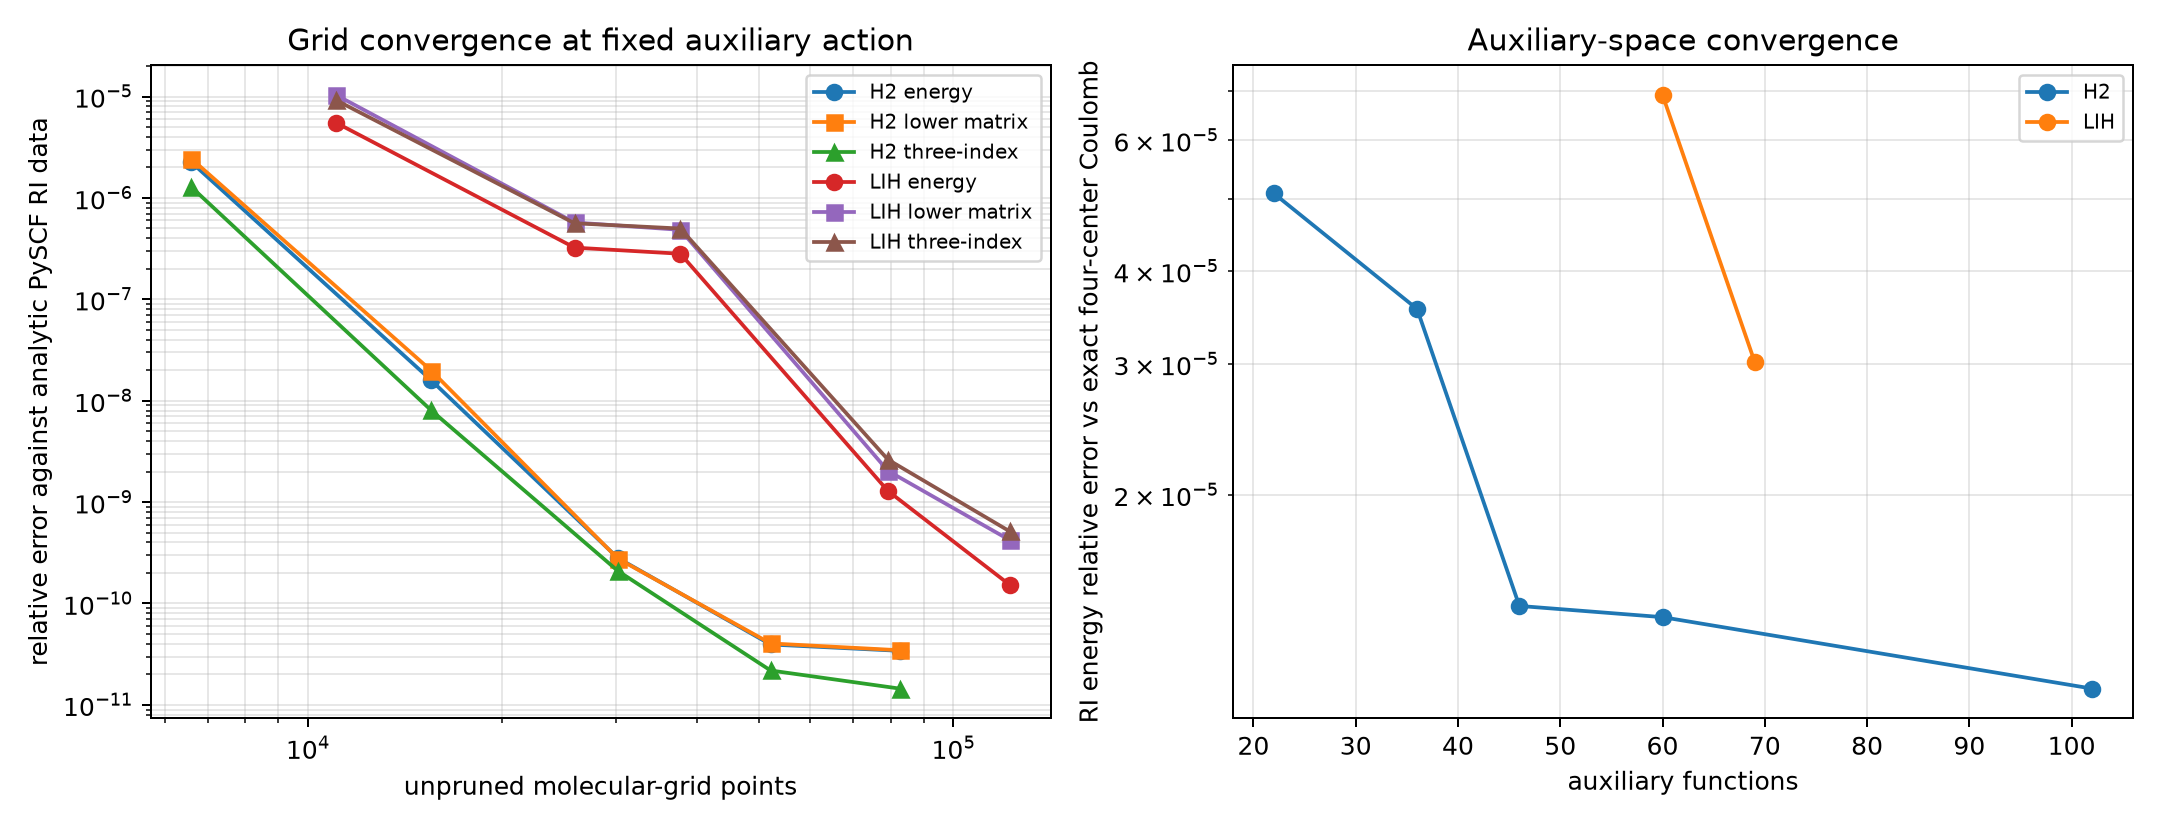
\includegraphics[width=0.88\textwidth]{figures/chapter13_nq9/nq2_grid_and_auxiliary_convergence.png}
  \caption{NQ2 grid and auxiliary-basis convergence.  The two axes are
  distinct approximation controls.}
  \label{fig:ri}
\end{figure}

The complete LDA source derivative closes to $3.64\times10^{-10}$ a.u. in
NQ5.  The CO/PBE source sequence has a useful central-difference window from
$3\times10^{-3}$ to $3\times10^{-2}$ and a best complete residual
$7.39\times10^{-9}$ a.u.  Finer steps amplify deterministic cancellation in
separately evaluated RI-Hartree energies.  Repeated transition-region values
are bitwise identical, excluding stochastic evaluator noise.  The PBE term
itself is at its symmetry floor for this CO direction; H$_3^+$ independently
tests a nonzero PBE source contribution.

\begin{figure}[htbp]
  \centering
  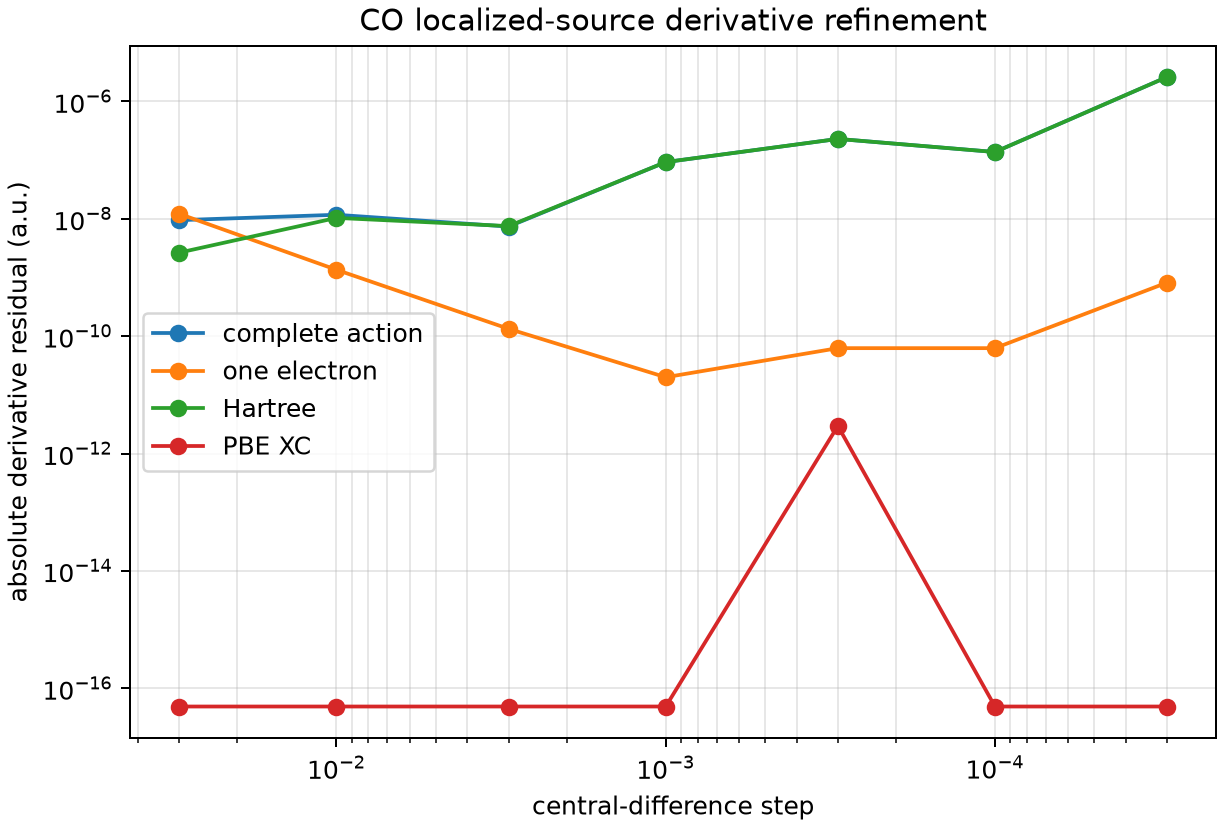
\includegraphics[width=0.82\textwidth]{figures/chapter13_nq9/nq8_co_source_refinement.png}
  \caption{CO localized-source central-difference refinement.  The upturn at
  small step is the resolved RI-Hartree subtraction floor.}
  \label{fig:co-source}
\end{figure}

\subsection{Dynamics, invariants, and power}

The NQ6 campaign contains 56 completed trajectories, 920 trajectory rows,
and 280 array archives.  The minimum measured final-density convergence
order is 3.7909.  Tightening the nonlinear tolerance changes the final
density by at most $7.46\times10^{-14}$ and the energy by
$4.94\times10^{-13}$ Ha, separating nonlinear iteration from timestep error.

At the finest step the maximum metric orthonormality, occupation-spectrum,
trace, and metric particle-number defects are respectively
$1.33\times10^{-11}$, $1.33\times10^{-11}$, $2.48\times10^{-12}$, and
$2.66\times10^{-11}$.  The real-space particle-number residual
$9.50\times10^{-9}$ is instead limited by the independently measured
level-4 spatial quadrature.  No metric correction was applied.

\begin{figure}[htbp]
  \centering
  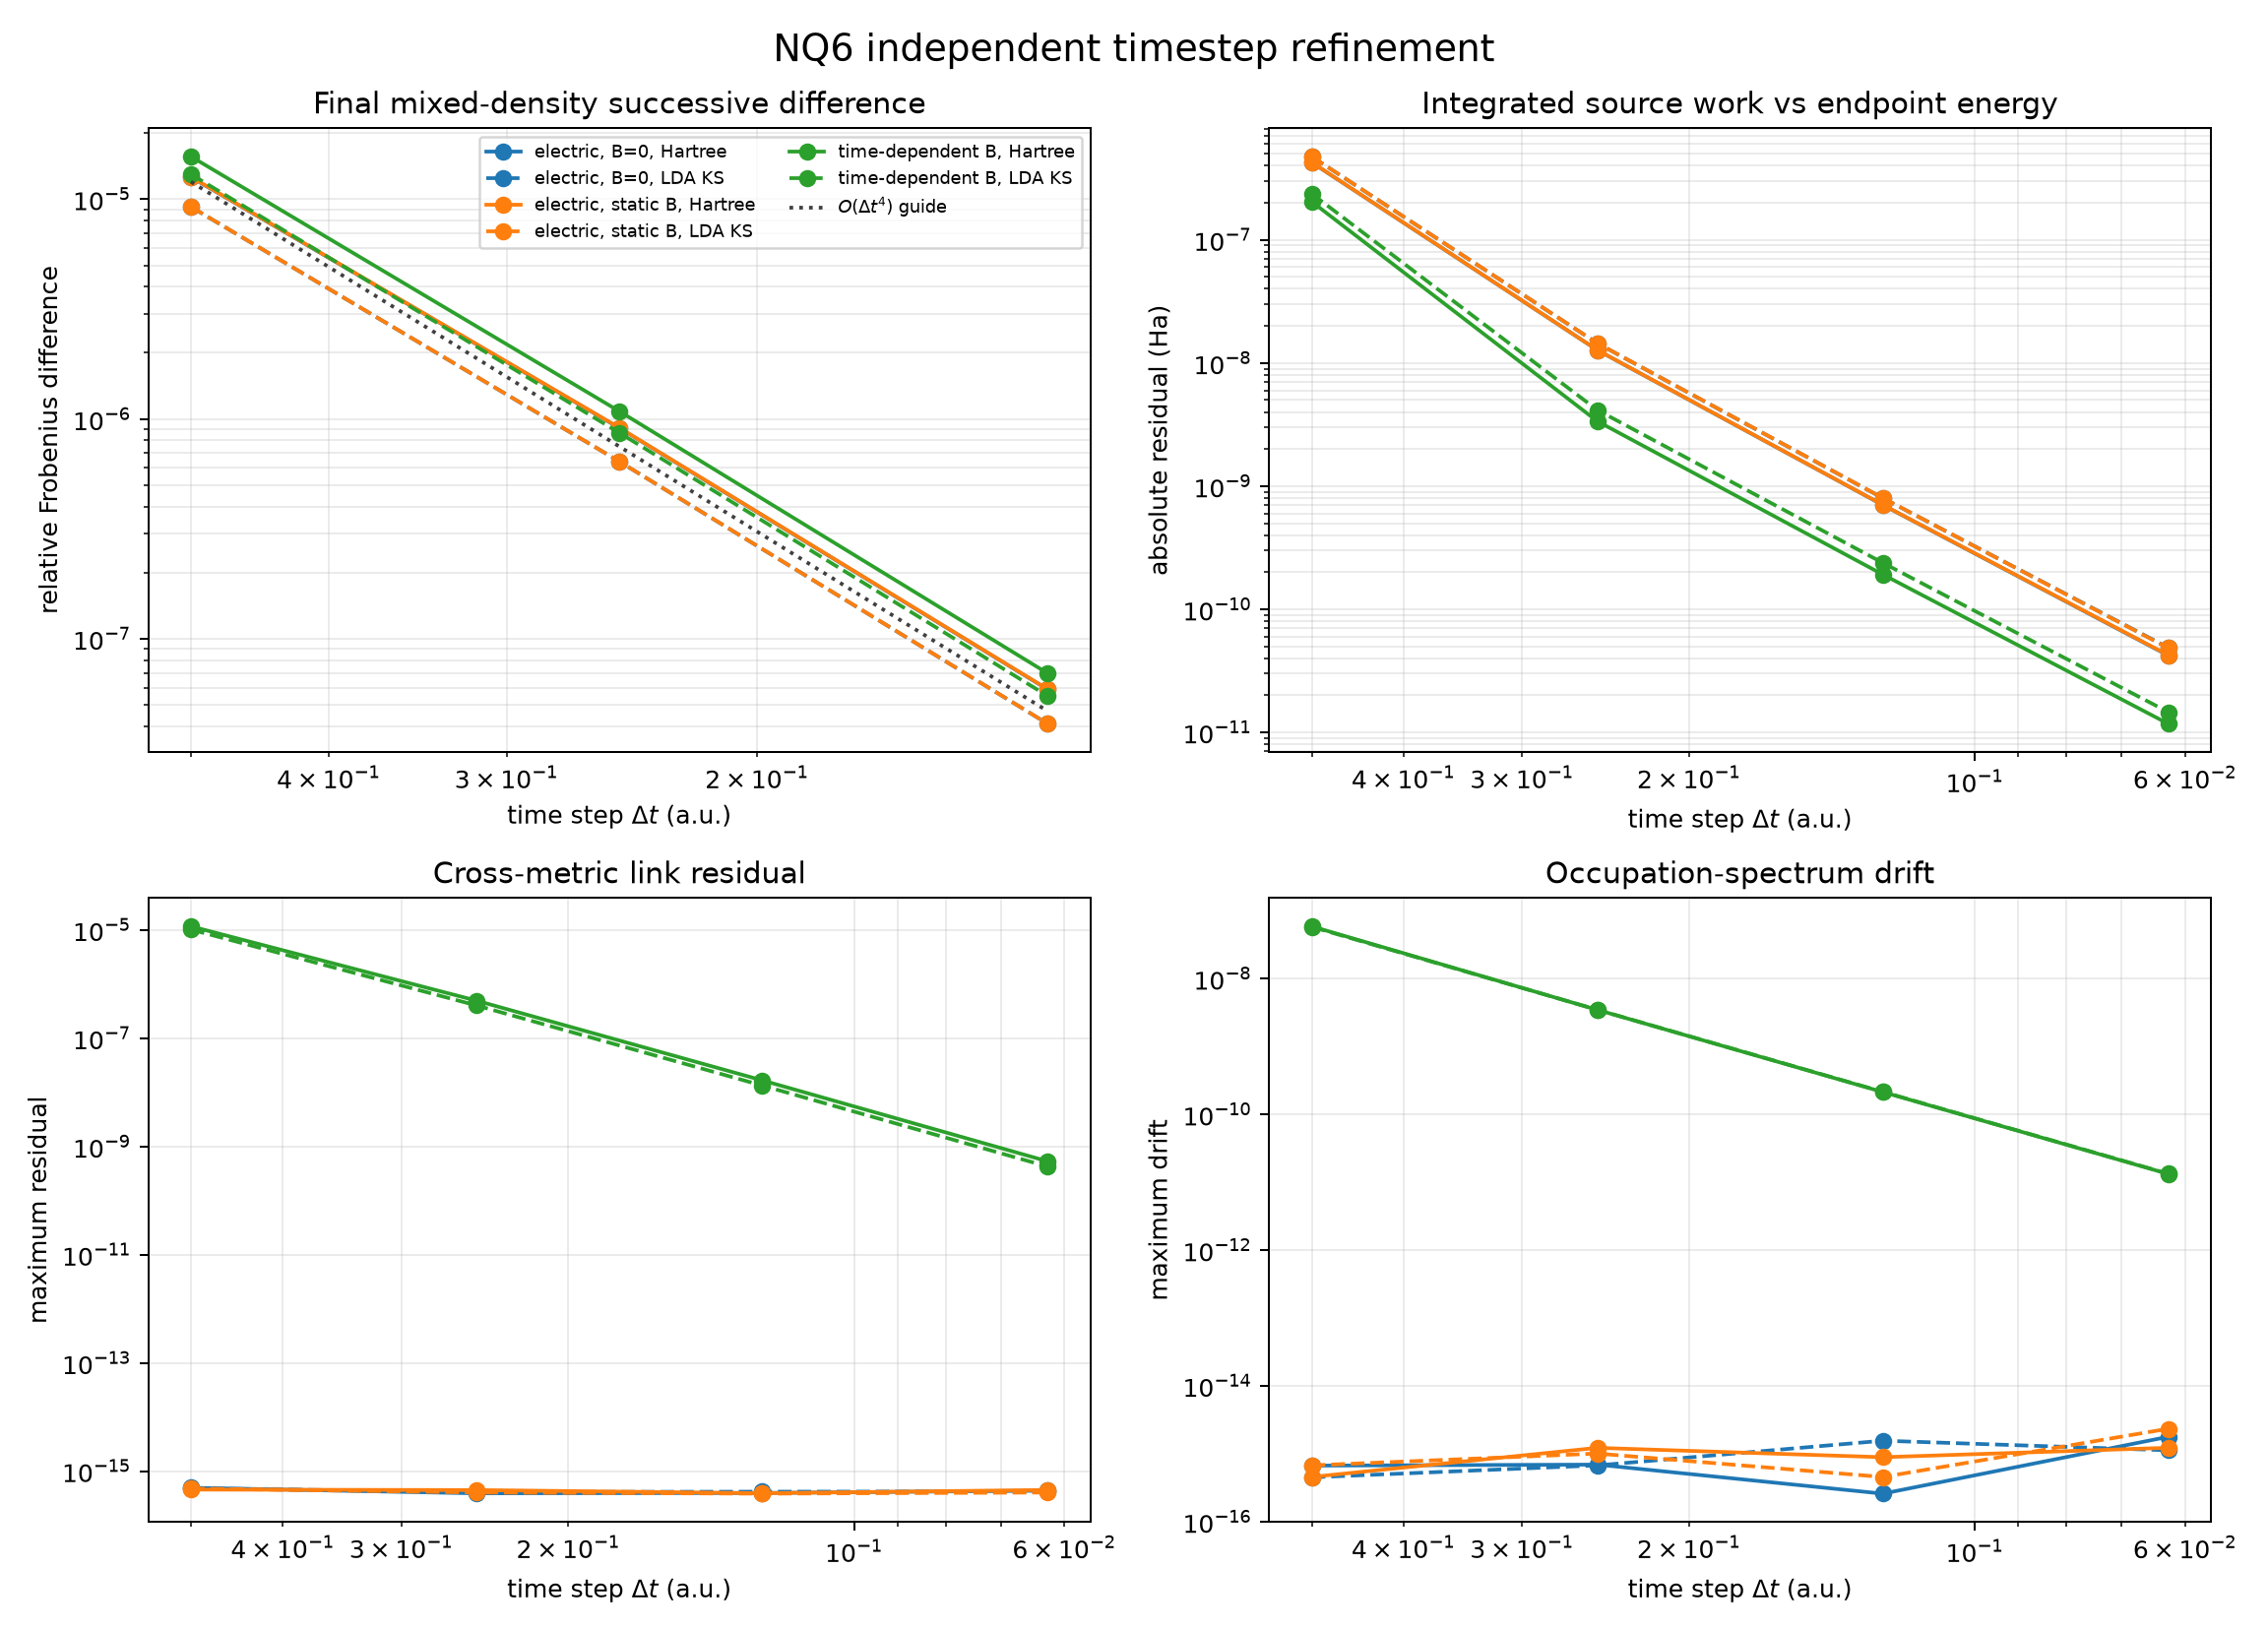
\includegraphics[width=0.88\textwidth]{figures/chapter13_nq9/nq6_timestep_convergence.png}
  \caption{Independent timestep convergence for the accepted nonlinear
  connection-aware propagator.}
  \label{fig:timestep}
\end{figure}

The finest instantaneous matrix/source power difference is
$3.25\times10^{-13}$ Ha/a.u.; the endpoint mechanical-energy versus integrated
source-work defect is $4.87\times10^{-11}$ Ha.  The PBE transfer trajectory
closes to $4.06\times10^{-10}$ Ha.  These are complete-action identities,
not comparisons to a current borrowed from another gauge or model.

\begin{figure}[htbp]
  \centering
  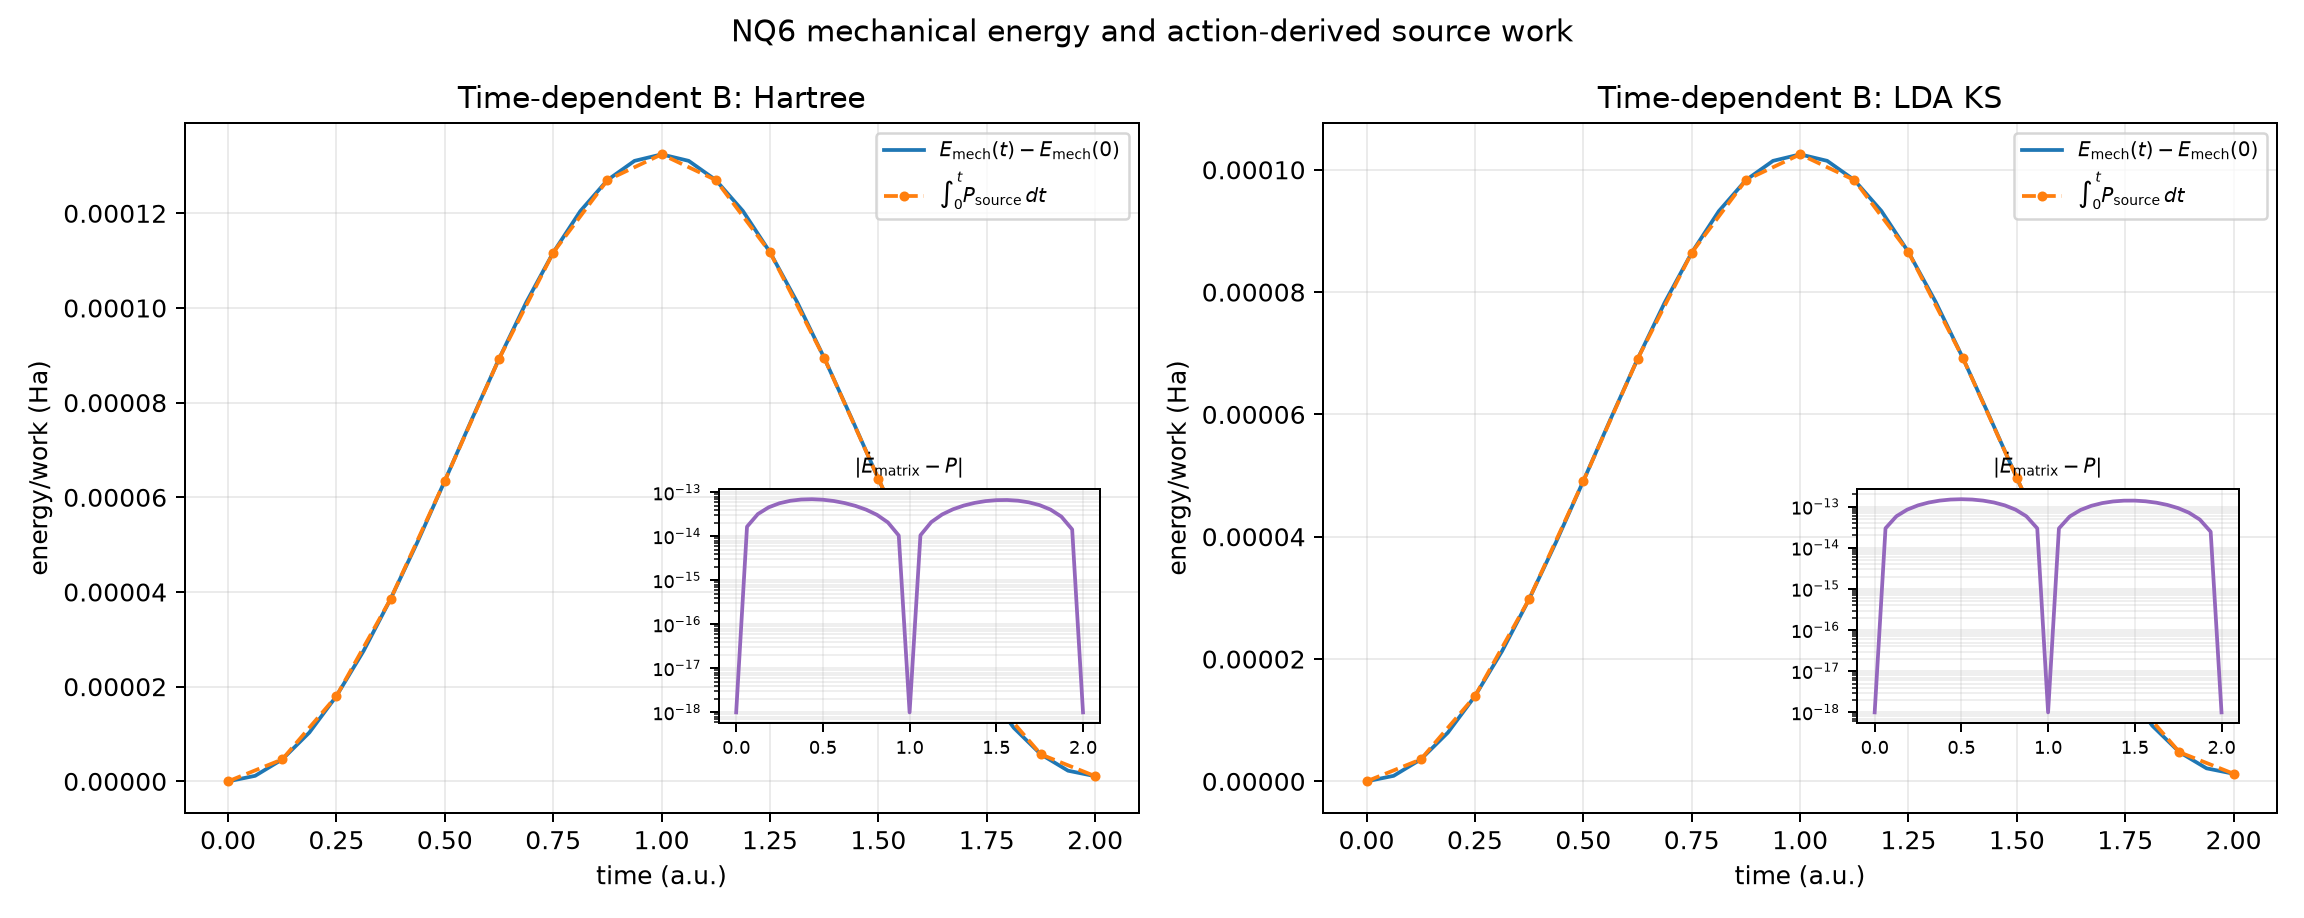
\includegraphics[width=0.88\textwidth]{figures/chapter13_nq9/nq6_induction_energy_work.png}
  \caption{Mechanical energy and integrated source work for the
  Maxwell-consistent magnetic-induction trajectory.}
  \label{fig:power}
\end{figure}

\section{Reduced-model decision and domain failures}

All reduced levels retain exact endpoint Wilson links but truncate the
endpoint-removed internal finite-spread action differently.  P0 deletes the
internal spread, E1 adds the first uniform-electric connection increment,
strict C1 consistently retains all degree-zero and degree-one terms, and the
density-resummed action evaluates unexpanded nonlinear closures on
$n_0+n_1$.  The last is a different action, not a repair of strict C1.

At zero magnetic field every reduced level recovers the exact action at the
stationary numerical floor.  E1 is exact for the tested zero-$B$ uniform
electric source: final density, energy trajectory, and power trajectory
errors are at most $6.59\times10^{-13}$, $3.74\times10^{-13}$, and
$1.01\times10^{-12}$.  At nonzero magnetic field, P0 state error is first
order while strict C1 is second order.  C1 improves stationary mixed density
by at least a factor 13.43 and dynamic final density over the better of P0/E1
by at least a factor 5.69.  The smallest C1 model-error to timestep-error ratio
is $6.79\times10^3$, so the comparison is physically resolved.

C1 does not uniformly improve every scalar energy or source-power coefficient.
This is a retained negative result: a better state and lower matrix do not
force every derivative of an omitted second-order action term to improve at
the same order.  Density-resummed C1 splits the sampled dynamic comparisons
evenly with strict C1 and extends no sampled domain.  Strict C1 is therefore
the accepted near-term reduced action only within this bounded LDA H$_3^+$
domain.

\begin{figure}[htbp]
  \centering
  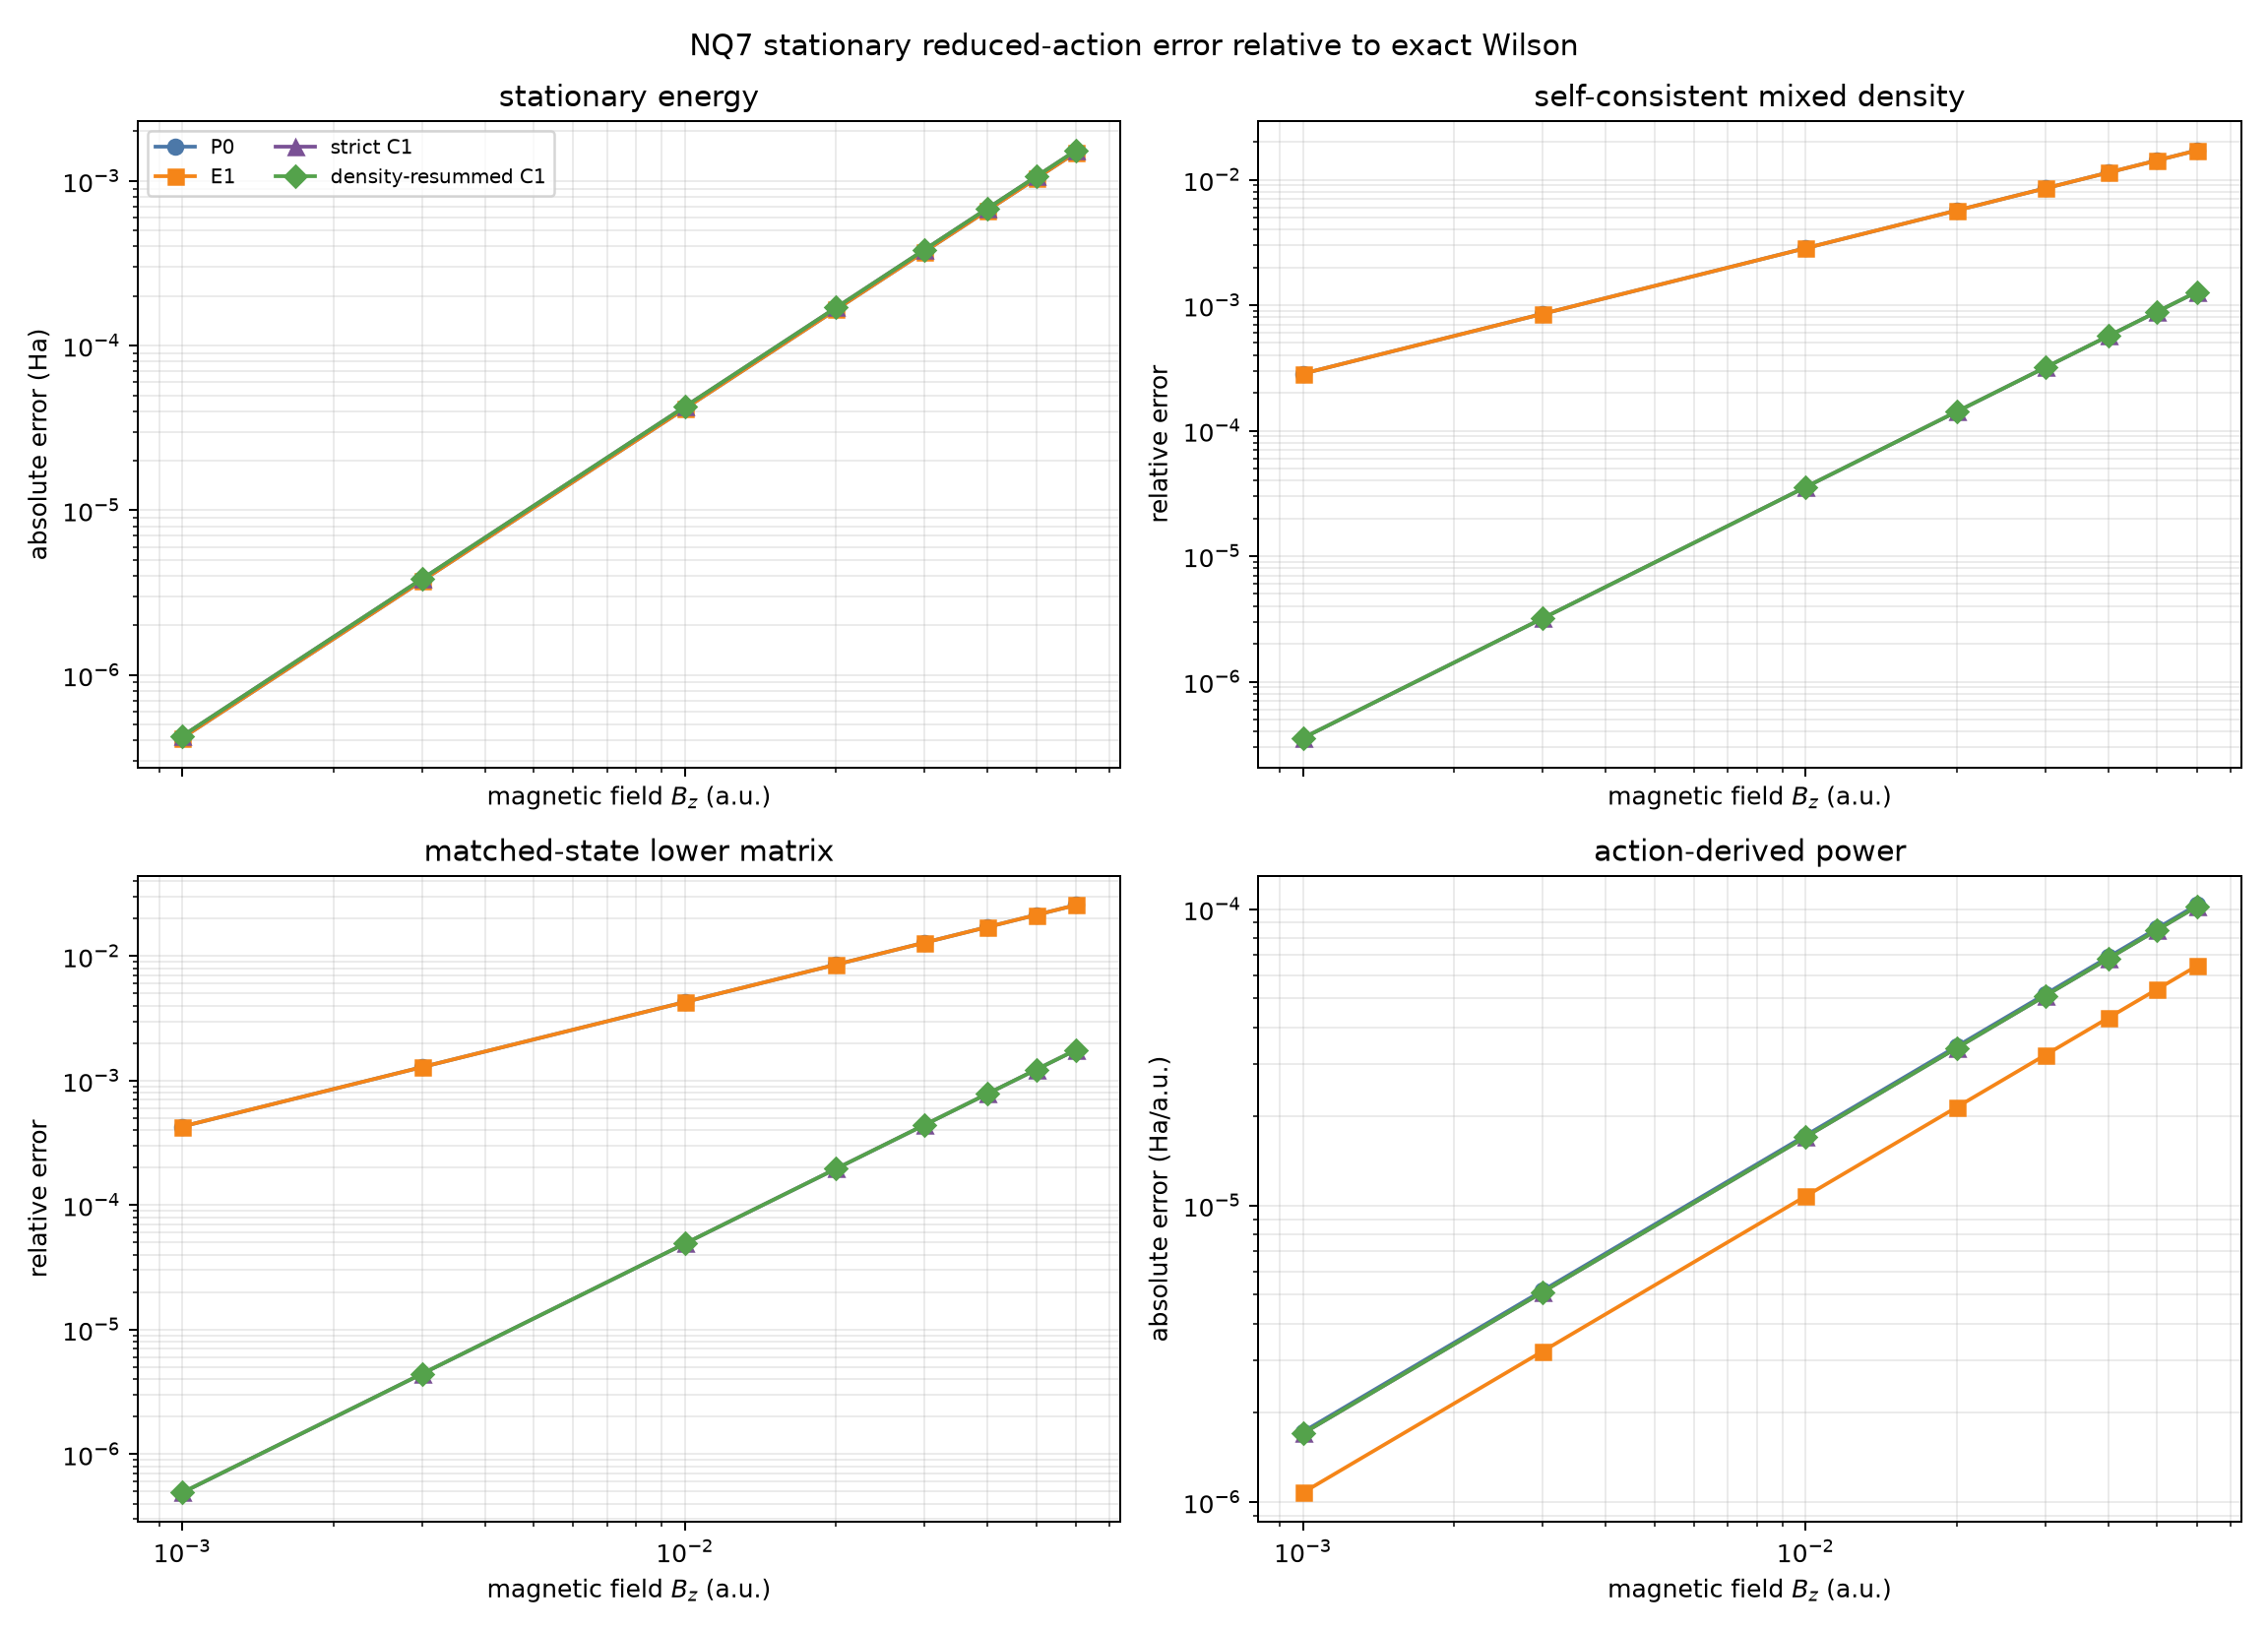
\includegraphics[width=0.88\textwidth]{figures/chapter13_nq9/nq7_stationary_field_errors.png}
  \caption{Stationary exact-versus-reduced errors.  Strict C1 removes the
  leading state and lower-matrix error, but not every scalar coefficient.}
  \label{fig:reduced}
\end{figure}

The decisive domain limitation is basis conditioned.  Every tested
aug-cc-pVDZ reduced level fails metric positivity at the first nonzero
sampled field $B_z=0.03$ a.u.; the independently recomputed exact Wilson
metric remains positive at every stress point.  Across the full stress scan,
48 reduced failures are visible and none is clipped, regularized, corrected,
or projected.  The scan brackets failure intervals; it does not locate a
continuous critical field and supports no molecule-independent cutoff.

\begin{figure}[htbp]
  \centering
  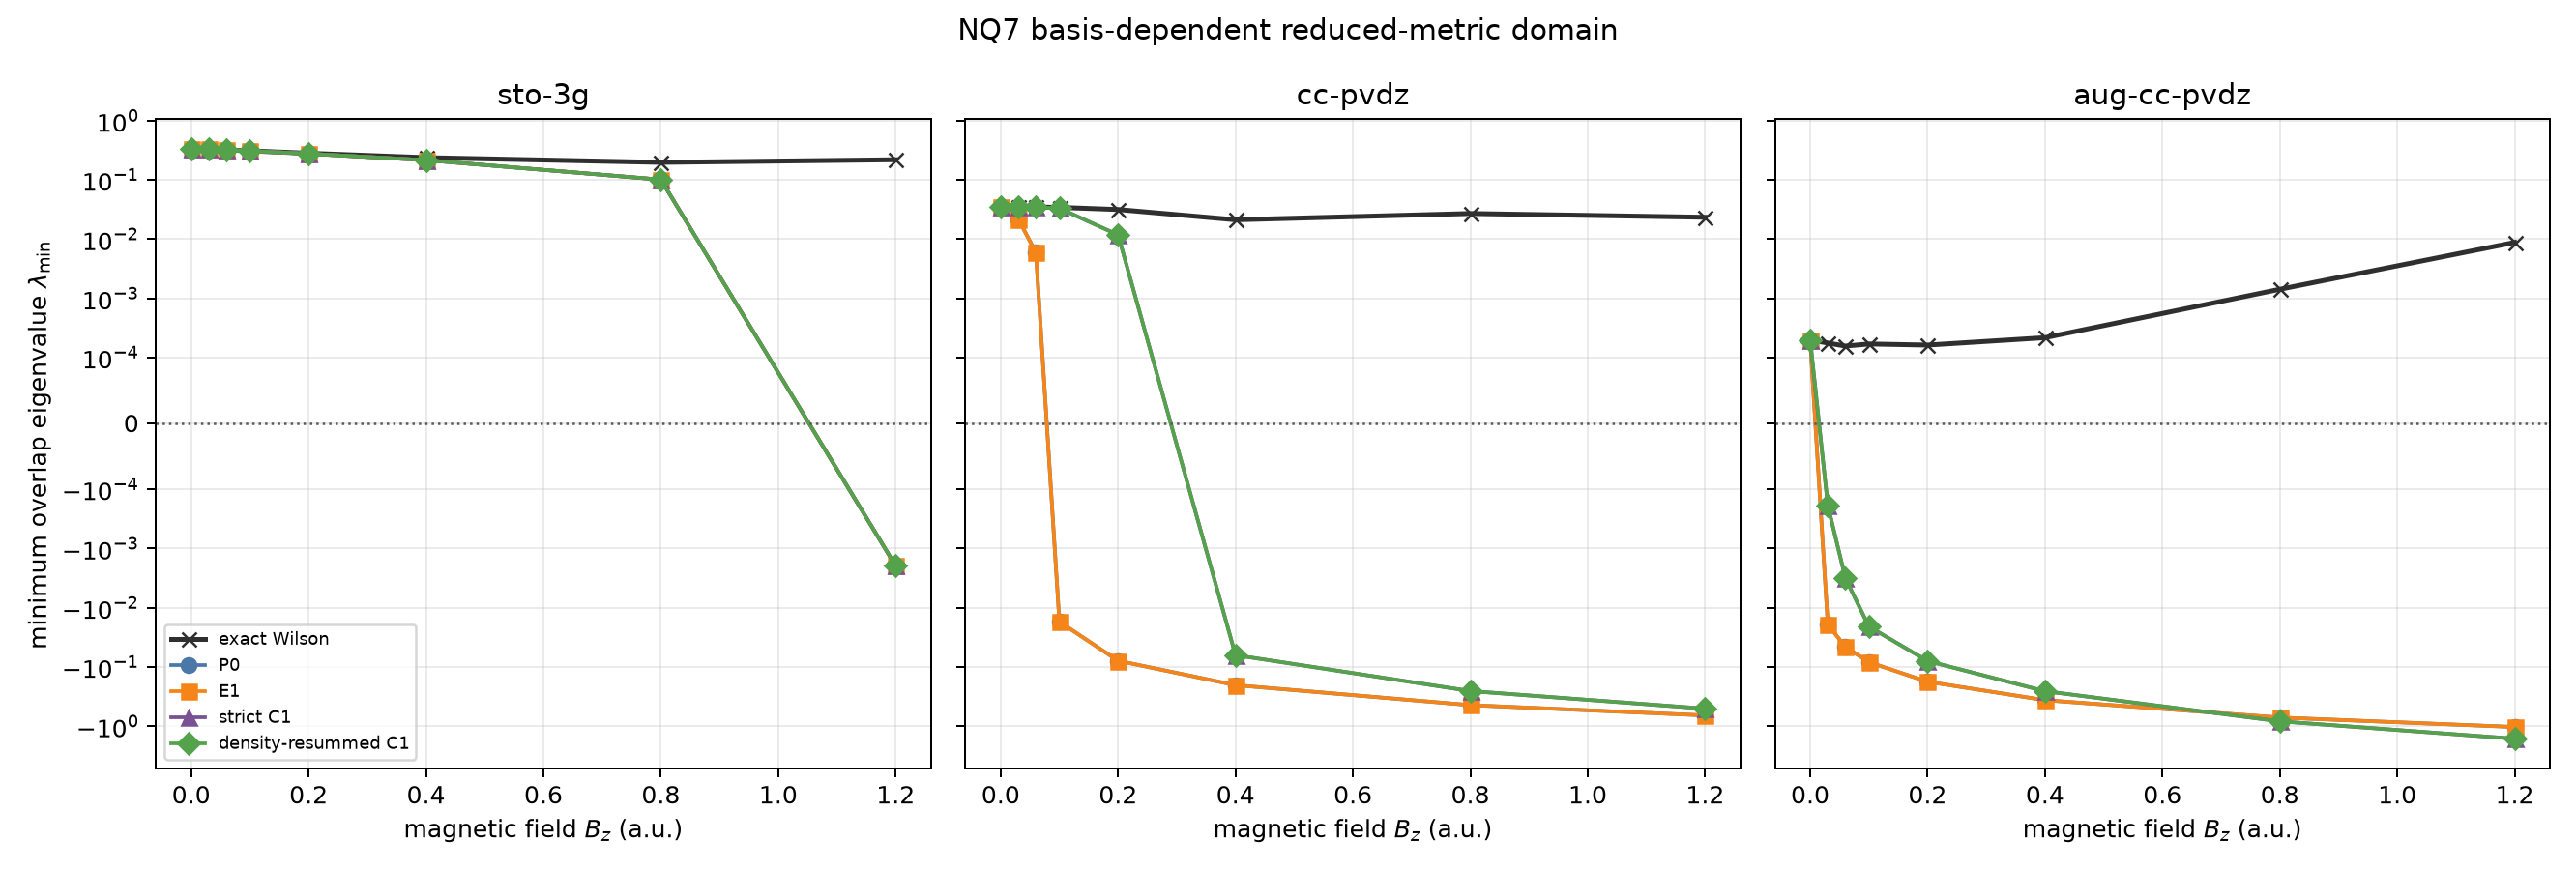
\includegraphics[width=0.88\textwidth]{figures/chapter13_nq9/nq7_domain_metric_boundaries.png}
  \caption{Basis-dependent reduced-metric domain boundaries.  The diffuse
  basis failure is a property of the truncation, not singularity of the exact
  Wilson overlap.}
  \label{fig:domain}
\end{figure}

\section{GGA and molecular transfer}

NQ8 introduces the separate \emph{quadrature--Wilson GGA} realization.  It
tests both $n_W$ and $\nabla n_W$ responses, same-grid PySCF/libxc agreement,
stationary states, sources, continuity, power, and short nonlinear propagation
for H$_3^+$ and closed-shell CO in cc-pVDZ/weigend on unpruned level-4 grids.
CO has 28 AOs, 106200 grid points, a peak density 297.701, and maximum density
gradient 4521.23, compared with 0.335 and 0.585 for H$_3^+$.  Nonzero C--O and
O--C lower-matrix blocks ensure that the transfer exercises compact core,
steep-gradient, and heteronuclear pair regions.

The maximum PBE transfer residuals are $2.37\times10^{-13}$ for weak
finite-region continuity, $6.43\times10^{-19}$ for global charge,
$3.56\times10^{-14}$ Ha/a.u. for instantaneous power,
$4.06\times10^{-10}$ Ha for endpoint work--energy balance, and
$2.01\times10^{-8}$ for the final-density difference between timesteps 0.05
and 0.025 a.u.  The transfer time is only 0.2 a.u.; it is not a spectroscopy
or long-time stability claim.  No reduced GGA P0/E1/C1 action is accepted.

\section{Negative and failed results}

The campaign retains failures as evidence rather than erasing them:

\begin{enumerate}
  \item the RI auxiliary basis produces a resolved $6.90\times10^{-5}$
        relative Hartree approximation error;
  \item NQ4 preserves an incomplete campaign, a complete but incorrectly
        labelled campaign, and a derivative-order fit contaminated by a
        floor-dominated point;
  \item the first NQ5 GPU invocation used the wrong launcher and failed two
        explicit device-contract assertions before the corrected run passed;
  \item a host power failure interrupted 33 of 56 NQ6 trajectories, forcing a
        clean rerun rather than a splice or undocumented resume;
  \item the preliminary NQ6 analysis used continuity and power thresholds
        below the measured quadrature floor and correctly failed;
  \item all sampled aug-cc-pVDZ reduced actions fail their metric domain at
        the first nonzero field, while exact Wilson remains regular;
  \item density-resummed C1 supplies no systematic improvement over strict C1;
  \item the CO source derivative reaches an RI energy-subtraction floor; and
  \item NQ8 preserves both a shell-appended non-scientific log hash mismatch
        and a superseded worst-sweep-point component criterion.
\end{enumerate}

The raw numerical NQ8 artifacts authenticate.  The final \path{run.log}
changed only because the outer shell appended completion text after the
Python process wrote provenance.  It is explicitly excluded from scientific
evidence rather than silently rehashed.

\section{Equation-to-code-to-evidence map}

\begin{longtable}{p{0.15\textwidth}p{0.27\textwidth}p{0.25\textwidth}p{0.09\textwidth}p{0.15\textwidth}}
\caption{Final compact traceability map.  Full rows, tests, scopes, and floors
are in \texttt{tables/equation\_code\_evidence.csv}.}\label{tab:traceability}\\
\toprule
Object & Mathematical role & Reusable implementation & Gates & Limiting evidence\\
\midrule
\endfirsthead
\toprule
Object & Mathematical role & Reusable implementation & Gates & Limiting evidence\\
\midrule
\endhead
Density & $n_W=P^{ij}\chi_i^W\chi_j^{W*}$ & \path{wilson_density.py} & NQ1,3,8 & factorization and grid floors\\
Hartree & $\frac12\rho^TJ^{-1}\rho$ and derivatives & \path{ri_wilson_hartree.py} & NQ2 & grid, auxiliary, rank, and solve scans\\
LDA & $\sum_gw_gf(n_g)$ and derivatives & \path{wilson_lda.py} & NQ3 & same-grid libxc and directions\\
GGA & $\sum_gw_gf(n_g,\nabla n_g)$ and derivatives & \path{wilson_gga.py} & NQ8 & same-grid PBE and CO transfer\\
Stationary & $K[P]C=SC\varepsilon$ & \path{wilson_stationary.py} & NQ4,8 & residual and gauge scans\\
Sources & fixed-history action derivative & \path{wilson_sources.py} & NQ5,8 & source sequences and decomposition\\
Ward and continuity & gauge identity and weak balance & \path{wilson_sources.py} & NQ5,6,8 & off-shell and trajectory tests\\
Connection & $S\dot C=-(\omega+\iu K/\hbar)C$ & \path{time_connection.py} & NQ6 & metric compatibility\\
Propagation & nonlinear Gauss--Magnus congruence & \path{tensorial.py} & NQ6--8 & timestep and nonlinear refinement\\
Power & $\Delta U=\int\langle j,E\rangle dt$ & \path{wilson_dynamics.py} & NQ6,8 & matrix, source, and endpoint work\\
Reduced models & P0, E1, strict/resummed C1 & \path{reduced_wilson.py} & NQ7 & exact comparisons and domain scan\\
\bottomrule
\end{longtable}

\section{Supported domain and exclusions}

The evidence supports one bounded statement:

\begin{quote}
The exact straight-Wilson finite molecular model, Coulomb-metric RI Hartree
closure, restricted pure-LDA and pure-PBE adiabatic actions, their variational
lower matrices and fixed-history weak sources, and connection-aware nonlinear
propagation form one numerically consistent implementation over the accepted
H$_2$, LiH, H$_3^+$, and CO fixtures.  Strict C1 is a controlled first-order
reduced working action inside the sampled pure-LDA H$_3^+$ domain, whose
basis-conditioned failures remain explicit.  The exact Wilson action remains
the reference.
\end{quote}

This statement does \emph{not} qualify moving nuclei, a nonadiabatic nuclear
connection, spatially nonuniform propagated fields, Maxwell backreaction,
periodic systems, pseudopotentials, spin polarization, hybrids, meta-GGAs,
nonlocal correlation, an exact interacting transverse current, reduced GGA
actions, long-time stability, spectroscopy, systematic basis convergence, or
broad chemical production use.

\section{Chapter 14 handoff}

The proposed Chapter 14 title is \emph{Numerical realization and
qualification of fixed-centre Wilson-projected adiabatic dynamics}.  Its
recommended sections are:

\begin{enumerate}
  \item scope, variables, index conventions, and realization tuple;
  \item exact Wilson density and variational Hartree/LDA/GGA actions;
  \item stationary nonlinear states and gauge/frame covariance;
  \item action-derived weak sources, Ward identity, and continuity;
  \item connection-aware nonlinear Gauss--Magnus propagation;
  \item mechanical energy, source power, and work balance;
  \item P0, E1, strict-C1, and resummed-C1 validity and failures;
  \item molecular and functional transfer from H$_2$/LiH/H$_3^+$ to CO/PBE;
  \item numerical error budget, negative results, and reproducibility; and
  \item bounded conclusions and open extensions.
\end{enumerate}

The detailed outline is in \path{docs/chapter13_nq9_chapter14_outline.md}.
It is a writing proposal only; NQ9 does not authorize edits to the formalism
book.

\section{Artifact index and reproduction}

The immutable NQ9 synthesis root is
\begin{quote}\small
\path{/home/cgs/00_WORK/Projection_Code/CALCULATIONS/campaigns/}\linebreak
\path{chapter13_wilson_adiabatic_qualification/}\linebreak
\path{nq9_synthesis_20260924T220919Z_74a493241667}.
\end{quote}
Its entry points are \path{result.json}, \path{provenance.json}, and
\path{completed.json}.  Derived tables include accepted gates, artifact
authentication, every accepted measurement, the full equation/code/evidence
map, all review limitations, explicit negative results, and the selected
figure manifest.

The nine accepted gate entry points are
\path{docs/chapter13_nq0_contract_and_field_free_reference.md} through
\path{docs/chapter13_nq8_gga_transfer_qualification.md}.  Their decisions are
in \path{docs/reviews/chapter13_nq0_review_20260921.json} through
\path{docs/reviews/chapter13_nq8_review_20260924.json}.  Those records contain
the immutable raw roots and primary hashes.

From a clean repository at commit \texttt{74a493241667}, reproduce the
synthesis with
\begin{verbatim}
env OMP_NUM_THREADS=2 OPENBLAS_NUM_THREADS=2 MKL_NUM_THREADS=2 \
  NUMEXPR_NUM_THREADS=2 VECLIB_MAXIMUM_THREADS=2 \
  /home/cgs/01_TOOLS/EasyBuild/conda/bin/conda run \
  -p /home/cgs/01_TOOLS/EasyBuild/conda/envs/aion \
  python tools/synthesize_chapter13_nq9.py \
  --repo /home/cgs/00_WORK/Projection_Code/aion \
  --output <new-empty-output-directory>
\end{verbatim}

The portable report figures are copied only after their synthesis hashes are
verified:
\begin{verbatim}
python tools/build_chapter13_nq9_report_assets.py \
  --synthesis <nq9-synthesis-root> \
  --output docs/figures/chapter13_nq9
\end{verbatim}
The report is compiled with two noninteractive \path{/usr/bin/pdflatex}
passes from \path{docs}; the compilation log is checked for LaTeX errors,
undefined references, and missing files.

\section{NQ9 review boundary}

The NQ9 synthesis is reconstructive: it finds no missing or mismatched
mandatory NQ0--NQ8 artifact and introduces no new physical calculation.  It
supports archival closure of Chapter 13 and the proposed Chapter 14 writing
handoff, subject to explicit user review.  Until that review is recorded,
NQ9 remains \status{executed\_unreviewed}.

\end{document}
